\section{System Architecture Overview}
\label{sec:4_1}

The fraud detection framework implements a modular pipeline architecture separating data processing, feature engineering, graph construction, model training, and real-time inference into distinct components.

\begin{figure}[htbp]
    \centering
    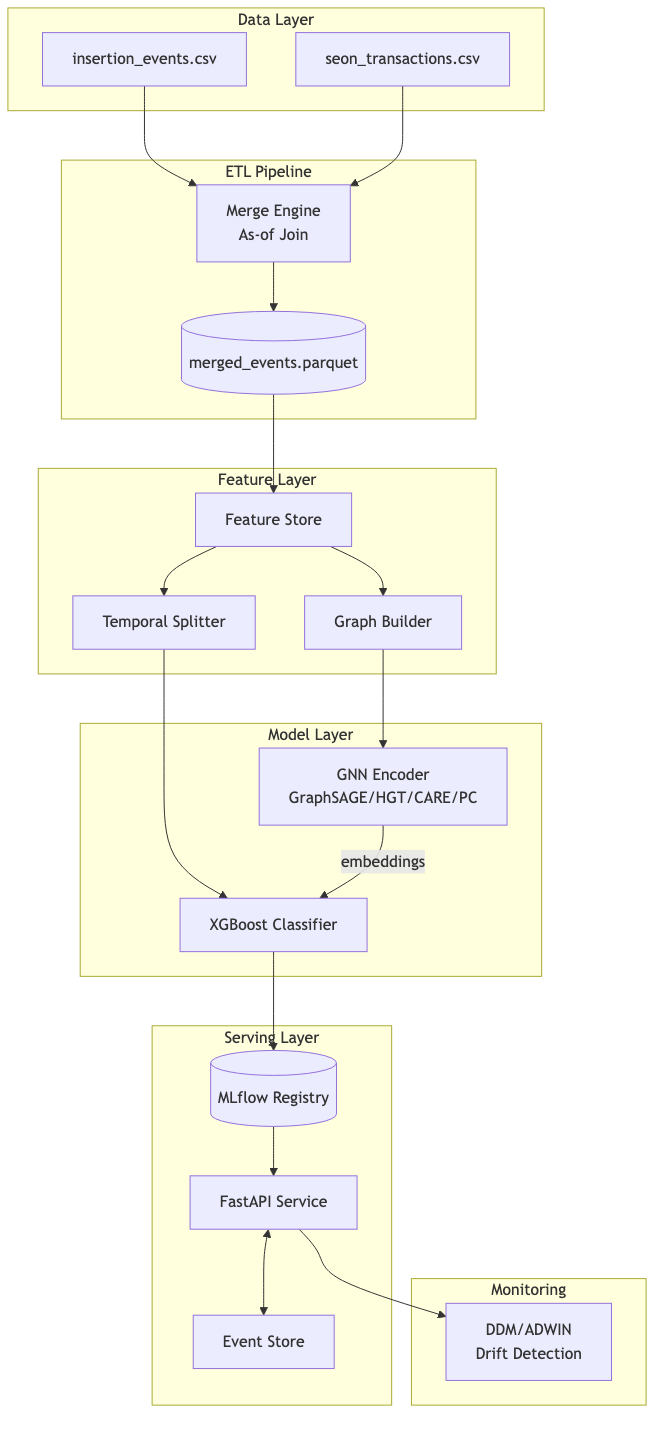
\includegraphics[width=1.1\textwidth,height=0.75\textheight,keepaspectratio]{figures/fig_4_4_1_1.png}
    \caption{System Architecture: Data Layer → ETL Pipeline → Feature Layer → Model Layer → Serving Layer}
    \label{fig:4_1}
\end{figure}

The architecture follows a layered design with single responsibility per component:

\textbf{Data Layer:} Ingests raw CSV files from SMG's data warehouse (\texttt{insertion\_events.csv} and \texttt{seon\_transactions.csv}). The data sources contain heterogeneous timestamp formats requiring standardization.

\textbf{ETL Pipeline:} Merges event and SEON data using temporal as-of joins implemented in Polars for memory-efficient processing. The pipeline handles streaming operations on 800K+ events, performing PII anonymization and temporal filtering. Output is stored in compressed Parquet format for downstream processing.

\textbf{Feature Layer:} Handles three critical operations: (1) feature extraction from merged data according to the feature schema, (2) temporal splitting with point-in-time label assignment and 7-day gap to prevent label leakage, and (3) heterogeneous graph construction with ~31M edges encoding device, IP, email, and phone relationships.

\textbf{Model Layer:} Implements a hybrid architecture where GraphSAGE extracts 16-dimensional node embeddings from the heterogeneous graph, which are concatenated with 65 base features and fed to an XGBoost classifier. Baseline models (Logistic Regression, Random Forest, vanilla XGBoost) are also implemented for comparison.

\textbf{Serving Layer:} Provides real-time inference through a FastAPI service with an internal event store enabling graph feature computation for incoming predictions. The API maintains a sliding window of recent events to construct graph connections for new listings.

\textbf{Monitoring:} Tracks prediction drift using DDM (Drift Detection Method) and ADWIN (Adaptive Windowing) algorithms to detect concept drift and trigger retraining.

All components are orchestrated through Hydra configuration management and tracked via MLflow experiment logging. The modular design enables independent testing and replacement of components for example, swapping GraphSAGE for CARE-GNN requires only configuration changes without pipeline modifications.

\subsection{Project Structure}

The implementation follows a modular organization separating concerns across distinct packages. The root directory contains two configuration folders: \texttt{conf/} for ETL pipeline configuration (including \texttt{config.yaml} and data settings) and \texttt{configs/} for training experiments (including hyperparameter optimization configurations for XGBoost and GNN+XGBoost variants). A \texttt{scripts/} directory contains orchestration scripts for running combined optimization workflows.

The core implementation resides in the \texttt{src/} package, organized into six functional modules:

\textbf{Key modules:}
\begin{itemize}
    \item \texttt{src/data/}: ETL pipeline with streaming support via Polars LazyFrames, containing modules for extraction (\texttt{extract.py}), transformation (\texttt{transform.py}), loading (\texttt{load.py}), and orchestration (\texttt{etl.py})
    \item \texttt{src/features/}: Feature schema definitions (\texttt{schema.py}), feature store (\texttt{store.py}), temporal splitting logic (\texttt{temporal\_split.py}), and heterogeneous graph construction (\texttt{graph\_builder.py})
    \item \texttt{src/models/}: Abstract base classes and concrete model implementations including baselines (\texttt{baselines.py}), XGBoost classifier (\texttt{xgboost\_classifier.py}), GraphSAGE implementation (\texttt{graphsage.py}), and hybrid architecture (\texttt{hybrid.py})
    \item \texttt{src/training/}: Single and expanding window training pipelines (\texttt{trainer.py}, \texttt{pipeline.py})
    \item \texttt{src/evaluation/}: SHAP explainability analysis (\texttt{shap\_analysis.py}) and drift detection algorithms (\texttt{drift.py})
    \item \texttt{src/api/}: FastAPI service (\texttt{main.py}) with in-memory event store (\texttt{store.py}) for real-time inference
\end{itemize}

This structure enables clear separation between data processing (\texttt{data/}), feature engineering (\texttt{features/}), model development (\texttt{models/}), and deployment (\texttt{api/}), facilitating independent testing and maintenance. The complete directory structure and implementation details are provided in Appendix~B.
